\documentclass[12pt]{article}
\usepackage{amsmath}
\usepackage{graphicx}
\usepackage{hyperref}
\usepackage[utf8]{inputenc}
\usepackage{geometry}
\usepackage{mathtools}
\usepackage{empheq}
\usepackage{listings}
\usepackage{xcolor}
\usepackage{minted}
\usepackage{svg}


\definecolor{LightGray}{gray}{0.9}

\graphicspath{ {./assets/} }
\geometry{margin=0.6in}

\title{CHEN 461 HW 6}
\author{Mark Levchenko}
\date{January 2023}

\begin{document}


\begin{enumerate}

% Problem 1 %%%%%%%%%%%%%%%%%%%%%%%%%%%%%%%%%%%%%%%%%%%%%%%%%%%%%%%%%%%%%%%%%%%%%%%%%%%
\newpage
\item Problem 6.13

\begin{align*}
    V \frac{dC_R}{dt} &= F (C_{R0} - C_R) - V k_1 C_R + V k_2 C_P - V k_3 C_R \\
    V \frac{dC_P}{dt} &= -F C_P + V k_1 C_R - V k_2 C_P \\
    \frac{dC_R}{dt} &= - \left(\frac{F}{V} + k_1 + k_3\right) C_R + k_2 C_P + \frac{F}{V} C_{R0} \\
    \frac{dC_P}{dt} &= k_1 C_R - \left(\frac{F}{V} + k_2\right) C_P \\
    y &= C_P \\
    A &= \begin{bmatrix}
        - \left(\frac{F}{V} + k_1 + k_3\right) & k_2 \\
        k_1 & - \left(\frac{F}{V} + k_2\right) \\
    \end{bmatrix} \\
    B &= \begin{bmatrix}
        \frac{F}{V} \\
        0 \\
    \end{bmatrix} \\
    C &= \begin{bmatrix}
        0 & 1 \\
    \end{bmatrix} \\
    D &= 0 \\
    G(s) &= c \left(s I - A\right)^{-1} b + d \\
    s I - A &= \begin{bmatrix}
        s + \left(\frac{F}{V} + k_1 + k_3\right) & - k_2 \\
        - k_1 & s + \left(\frac{F}{V} + k_2\right) \\
    \end{bmatrix} \\
    \mathrm{Adj}(s I - A) &= \begin{bmatrix}
        s + \left(\frac{F}{V} + k_2\right) & k_2 \\
        k_1 & s + \left(\frac{F}{V} + k_1 + k_3\right) \\
    \end{bmatrix} \\
    \mathrm{det}(s I - A) &= \left(s + \left(\frac{F}{V} + k_1 + k_3\right)\right) \left(s + \left(\frac{F}{V} + k_2\right)\right) - k_1 k_2 \\
    \mathrm{det}(s I - A) &= \left(s + \frac{F}{V} + k_1 + k_3\right) \left(s + \frac{F}{V} + k_2\right) - k_1 k_2 \\
    \theta &= \mathrm{det}(s I - A) \\
    \left(s I - A\right)^{-1} &= \theta^{-1} \begin{bmatrix}
        s + \left(\frac{F}{V} + k_2\right) & k_2 \\
        k_1 & s + \left(\frac{F}{V} + k_1 + k_3\right) \\
    \end{bmatrix} \\
    G(s) &= c \theta^{-1} \begin{bmatrix}
        s + \left(\frac{F}{V} + k_2\right) & k_2 \\
        k_1 & s + \left(\frac{F}{V} + k_1 + k_3\right) \\
    \end{bmatrix} \begin{bmatrix}
        \frac{F}{V} \\
        0 \\
    \end{bmatrix} \\
    G(s) &= c \theta^{-1} \begin{bmatrix}
        \frac{F}{V} \left(s + \left(\frac{F}{V} + k_2\right)\right) \\
        \frac{F}{V} k_1 \\
    \end{bmatrix} \\
    G(s) &= \theta^{-1} \begin{bmatrix}
        0 & 1 \\
    \end{bmatrix} \begin{bmatrix}
        \frac{F}{V} \left(s + \left(\frac{F}{V} + k_2\right)\right) \\
        \frac{F}{V} k_1 \\
    \end{bmatrix} \\
    G(s) &= \frac{\frac{F}{V} k_1}{\theta} \\
    G(s) &= \frac{\frac{F}{V} k_1}{\left(s + \frac{F}{V} + k_1 + k_3\right) \left(s + \frac{F}{V} + k_2\right) - k_1 k_2}
\end{align*}


% Problem 2 %%%%%%%%%%%%%%%%%%%%%%%%%%%%%%%%%%%%%%%%%%%%%%%%%%%%%%%%%%%%%%%%%%%%%%%%%%%
\newpage
\item Problem 6.7
\begin{align*}
    \intertext{State space model:}
    A_1 \frac{dh_1}{dt} &= F_{in} - \frac{h_1 - h_2}{R_1} \\
    A_2 \frac{dh_2}{dt} &= \frac{h_1 - h_2}{R_1} - \frac{h_2}{R_2} \\
    \intertext{Assume $R_1 = R_2 = 1$}
    \frac{dh_1}{dt} &= - \frac{h_1}{A_1} + \frac{h_2}{A_1} + \frac{F_{in}}{A_1} \\
    \frac{dh_2}{dt} &= \frac{h_1}{A_2} - \frac{2 h_2}{A_2} \\
    A &= \begin{bmatrix}
        - \frac{1}{A_1} & \frac{1}{A_1} \\
        \frac{1}{A_2} & - 2 \frac{h_2}{A_2} \\
    \end{bmatrix} \\
    B &= \begin{bmatrix}
        \frac{1}{A_1} \\
        0 \\
    \end{bmatrix} \\
    D &= 0 \\
    y &= h_2 \\
    & \text{Or,} \\
    y &= h_1 \\
    \intertext{Finding $h_2$}
    C &= \begin{bmatrix}
        0 & 1 \\
    \end{bmatrix} \\
    \intertext{Finding $h_1$}
    C &= \begin{bmatrix}
        1 & 0 \\
    \end{bmatrix} \\
\end{align*}

% Problem 3 %%%%%%%%%%%%%%%%%%%%%%%%%%%%%%%%%%%%%%%%%%%%%%%%%%%%%%%%%%%%%%%%%%%%%%%%%%%
\newpage
\item Problem 6.8
\begin{enumerate}
    \item 
    \begin{align*}
        \tau_1 \frac{dx_1}{dt} + x_1 &= ku \\
        \tau_2 \frac{dx_2}{dt} + x_2 &= kx_1 \\
        \frac{dx_1}{dt} &= \frac{-1}{\tau_1} x_1 + \frac{k}{\tau_1} u \\
        \frac{dx_2}{dt} &= \frac{k}{\tau_2} x_1 - \frac{1}{\tau_2} x_2 \\
        A &= \begin{bmatrix}
            \frac{-1}{\tau_1} & 0 \\
            \frac{k}{\tau_2} & \frac{-1}{\tau_2} \\
        \end{bmatrix} \\
        B &= \begin{bmatrix}
            \frac{k}{\tau_1} \\
            0 \\
        \end{bmatrix} \\
        C &= \begin{bmatrix}
            0 & 1 \\
        \end{bmatrix} \\
        D &= 0 \\
        sI - A &= \begin{bmatrix}
            s + \frac{1}{\tau_1} & 0 \\
            -\frac{k}{\tau_2} & s + \frac{1}{\tau_2} \\
        \end{bmatrix} \\
        \mathrm{Adj}(sI - A) &= 
        \begin{bmatrix}
            s + \frac{1}{\tau_2} & 0 \\
            \frac{k}{\tau_2} & s + \frac{1}{\tau_1} \\
        \end{bmatrix} \\
        \mathrm{det}(sI - A) &= \left(s + \frac{1}{\tau_2}\right) \left(s + \frac{1}{\tau_1}\right) \\
        (sI - A)^{-1} &= 
        \begin{bmatrix}
            \frac{s + \frac{1}{\tau_2}}{\left(s + \frac{1}{\tau_2}\right) \left(s + \frac{1}{\tau_1}\right)} & 0 \\
            \frac{\frac{k}{\tau_2}}{\left(s + \frac{1}{\tau_2}\right) \left(s + \frac{1}{\tau_1}\right)} & \frac{s + \frac{1}{\tau_1}}{\left(s + \frac{1}{\tau_2}\right) \left(s + \frac{1}{\tau_1}\right)} \\
        \end{bmatrix} \\
        (sI - A)^{-1} &= 
        \begin{bmatrix}
            \frac{\tau_1}{\tau_1 s + 1} & 0 \\
            \frac{k \tau_1}{\left(\tau_2 s + 1\right) \left(\tau_1 s + 1\right)} & \frac{\tau_2}{\tau_2 s + 1} \\
        \end{bmatrix} \\
    \end{align*}
\end{enumerate}


% Problem 4 %%%%%%%%%%%%%%%%%%%%%%%%%%%%%%%%%%%%%%%%%%%%%%%%%%%%%%%%%%%%%%%%%%%%%%%%%%%
\newpage
\item Problem 6.8 MATLAB

The purpose of this problem is to use MATLAB as a matrix calculator.

You will use the matrix operations and matrix functions in MATLAB, including the expm function for the matrix exponential.

Consider the CSTR example of p. 172, with state equation given by Eq. (6.1.5), where F = 10 $l$/min, V = 100 $l$, k$_1$ = 0.1 min$^{-1}$, k$_2$ = 0.05 min$^{-1}$, k$_3$ = 0.02 min$^{-1}$

a) How are the input and state vector related at steady state? If the inlet concentration of the reactant is steady and equal to C$_{R0,s}$ =2 mol/$l$, calculate the corresponding steady state values of C$_R$, C$_I$ and C$_P$.

b) Use formulas from Table 6.2 (p. 188) and Table 6.3 (p.190) to calculate and plot

• the response of C$_R$, C$_I$ and C$_P$ to a step change in C$_{R0}$ of size M = 2 mol/$l$

• the response of C$_R$, C$_I$ and C$_P$ to a ramp change in C$_{R0}$ of slope M = 0.5 mol/min

• the response of C$_P$ to a sinusoidal change in C$_{R0}$ of amplitude M = 1 mol/$l$ and frequency $\omega$= 0.2 min$^{-1}$ all in deviation form.

c) Calculate the zero-order hold discretization of the system (Eqns. (6.7.5) and (6.7.6) on p. 193) for sampling period T$_s$ = 0.2 min.

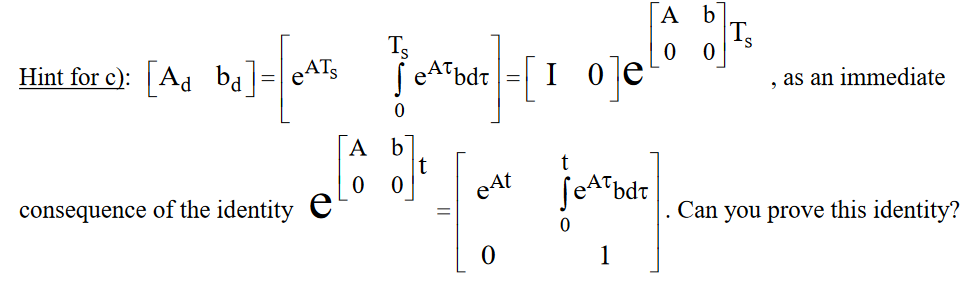
\includegraphics[width=0.8\textwidth]{assets/p4hint.png}

\end{enumerate}
\end{document}